%----------------------------------------------------------------------------------------
%	PACKAGES AND OTHER DOCUMENT CONFIGURATIONS
%----------------------------------------------------------------------------------------
\documentclass[a4paper, 12pt]{article}
%%%%%%%%%%%%%%%%%%%%%
%\usepackage{fullpage}
%\usepackage{setspace}
%\doublespacing
%%%%%%%%%%%%%%%%%%%%%
%\usepackage[margin=1in]{geometry}
%\usepackage[normalem]{ulem} % For striking out text
\usepackage{tikz}
\usepackage{natbib}
\usepackage{hyperref}
\definecolor{ref}{rgb}{0.0, 0.5, 1.0}
\hypersetup{colorlinks = true, allcolors = ref}
\usetikzlibrary{
    shapes,
    arrows,
    positioning,
    calc,
    fit,
    chains,
    fit,
    shapes,
    backgrounds}
%--------------------
%\newcommand{\note}[1]{%
%	\color{red}%
%	(\textbf{Note: }%
%	#1)%
%	\color{black}
%}
%--------------------
%--------------------
%\newcommand{\cancel}[1]{%
%	\color{red}%
%	\sout{#1}%
%	\color{black}
%}
%--------------------
\newcommand*{\xmin}{1}%
\newcommand*{\xmax}{2}%
\newcommand*{\ymin}{1}%
\newcommand*{\ymax}{9}%

\newcommand*{\xMin}{0.5}%
\newcommand*{\xMax}{2.5}%
\newcommand*{\yMin}{0.5}%
\newcommand*{\yMax}{9.5}%

%\pgfmathsetseed{3442}
\pgfmathsetseed{\number\pdfrandomseed}

%------------------------------------------------------------------


%----------------------------------------------------------------------------------------
\begin{document}


%\vfill
%\hfill
%\vspace{1cm}


\begin{center}
{\large \textbf{Grid Cellular Automaton:}\\\vspace{.5cm}
\textit{Documentation}}
\end{center}

\vspace{2cm}


%\begin{minipage}{0.45\textwidth}
%	\begin{flushleft}
%		{\textbf{Author}\\
%		Timothe van Meter$^1$\\\vspace{.15cm}
%		\footnotesize{$^1$\textit{Department of Biological Sciences,\\University of Illinois at Chicago, IL, USA}}\\\vspace{-.1cm}
%            \href{mailto:tvanme2@uic.edu}{tvanme2@uic.edu}}
%	\end{flushleft}
%\end{minipage}
%~
%\begin{minipage}{0.45\textwidth}
%	\begin{flushright}
%		\textbf{PhD Advisors:}\\
%		Dr. David Wise$^1$\\ % Supervisor's name\\
%            Dr. Jordi Moya-Larano$^2$\\\vspace{.15cm}
%            \footnotesize{$^2$\textit{Estacion Experimental de Zonas Aridas,\\CSIC, Almeria, SPAIN}}
%	\end{flushright}
%\end{minipage}

%\vspace{1cm}
%\newpage

%----------------------------------------------------------------------------------------
%	TEXT BODY
%----------------------------------------------------------------------------------------


% During my preliminary examination on the 8th of May 2020 the committee members (Drs. Gonzalez-Meler, Minor, Zellner, Moya-Laraño, Wise) suggested that several aspects of my project could be improved. This, either conceptually or logistically. I present the aspects of the project that were put in question during the preliminary examination, and for each I propose a solution and the developments that could be made in the future.



\subsection*{Parameter space exploration}

The following may be trivial for most of those who already are familiar with parameter exploration. In which case this entire section can be skipped.\newline\newline

The file \texttt{wrapper.c} calculates the number of simulations necessary to explore every unique combination of parameter values. The possible values for a parameter are specified by the user through the maximum ($i_{max}$), the minimum ($i_{min}$) and the increment in value ($i_{step}$) of that parameter. The number of total simulations to perform, N , is simply the product of the cardinal of each parameter that the user wants to vary in the simulations, i.e. the cardinal is the total number of distinct values a parameter can take.

$$ N = \prod_{i}^{P} \frac{ i_{max} - i_{min} }{ i_{step} } + 1 $$

With $P$ the number of variable parameters to include in the simulations and $ i_{max} \geq i_{min} , i_{step} \neq 0 $.\\

The value $N$ only provides us with the total number of simulations necessary to explore the entire parameter space, however it does not provide us with a method to list the parameter values so that all combinations are presented only once. 
Before presenting in details the method adopted here I explicit in which sense I use certain words. To explore the cardinal of one parameter, all of its possible value, as defined by its maximum ($i_{max}$), the minimum ($i_{min}$) and the increment in value ($i_{step}$); we proceed as following:
$\bullet$ The first value is $i_{min}$.\\
$\bullet$ All the posterior values are obtained by adding $i_{step}$ to the current value (incrementing) until $i_{max}$ is reached.\\
The above will be further referred as the \textit{ordered cardinal} of a parameter.\newline\newline


\begin{figure}[!h]
  \centering
  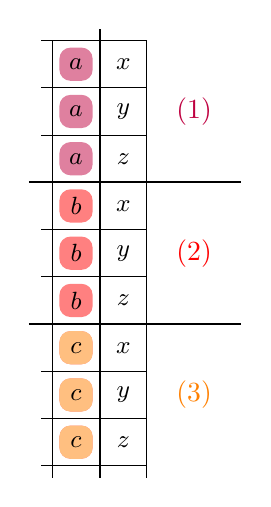
\begin{tikzpicture}[scale=.6]
    \foreach \i in {\xMin,...,\xMax} {
      \draw [black] (\i,\yMin) -- (\i,\yMax);
      \draw [black] (\i,\yMin) -- ($ (\i,\yMin) + (0,-.25) $);
    }
    \foreach \i in {\yMin,...,\yMax} {
      \draw [black] (\xMin,\i) -- (\xMax,\i);
      \draw [black] (\xMin,\i) -- ($ (\xMin,\i) + (-.25,0) $);
    }
    \foreach \x in {\xmin,...,\xmax} {
      \foreach \y in {\ymin,...,\ymax} {
        \ifnum \x < 2
        \ifnum \y > 6
        \node[fill=purple!50,inner sep=6pt,rounded corners] at (\x,\y) {};
        \else
        \fi
        \ifnum 7 > \y > 3 
        \node[fill=red!50,inner sep=6pt,rounded corners] at (\x,\y) {};
        \else
        \fi
        \ifnum \y < 4 
        \node[fill=orange!50,inner sep=6pt,rounded corners] at (\x,\y) {};
        \else
        \fi
        \else
        \fi
      }
    }
    \draw [black] (\xMin,\yMin) -- (\xMax,\yMin) -- (\xMax,\yMax) -- (\xMin,\yMax) -- (\xMin,\yMin);
    \node[] at (2,9) {\small{$x$}};
    \node[] at (2,8) {\small{$y$}};
    \node[] at (2,7) {\small{$z$}};
    \node[] at (2,6) {\small{$x$}};
    \node[] at (2,5) {\small{$y$}};
    \node[] at (2,4) {\small{$z$}};
    \node[] at (2,3) {\small{$x$}};
    \node[] at (2,2) {\small{$y$}};
    \node[] at (2,1) {\small{$z$}};
    \draw [thick, black] (0, 6.5) -- (4.5, 6.5);
    \node[purple] at (3.5,8) { $(1)$ };
    \draw [thick, black] (0, 3.5) -- (4.5, 3.5);
    \node[red] at (3.5,5) { $(2)$ };
    \draw [thick, black] (1.5, 0.25) -- (1.5, 9.75);
    \node[orange] at (3.5,2) { $(3)$ };
    \node[] at (1,9) {\small{$a$}};
    \node[] at (1,8) {\small{$a$}};
    \node[] at (1,7) {\small{$a$}};
    \node[] at (1,6) {\small{$b$}};
    \node[] at (1,5) {\small{$b$}};
    \node[] at (1,4) {\small{$b$}};
    \node[] at (1,3) {\small{$c$}};
    \node[] at (1,2) {\small{$c$}};
    \node[] at (1,1) {\small{$c$}};
    
  \end{tikzpicture}
  \label{fig:filling_method}
  \caption{vevzV }
\end{figure}

To explore the total parameter space the method orders all the variable parameters in a table and increments a parameter each time the next one has completely explored its cardinal once. This method is illustrated for two parameters, which are the two columns in Figure \ref{fig:filling_method} below. Both parameters haves three possible values $a$, $b$ and $c$ for the first parameter, and $x$, $y$ and $z$ for the second parameter. The total number of necessary simulations is thus, $N = 3 \cdot 3 = 9$, which corresponds to the number of lines in Figure \ref{fig:filling_method}. The parameter's cardinal are explored from the last column to the first. In Figure \ref{fig:filling_method} the first parameter's value is incremented only once the second parameter has completely explored its cardinal. The latter process is highligthed in the Figure with a different color code for each exploration of the second parameter's cardinal and the subsequent increment of the first parameter: in \color{purple}purple\color{black}, \color{red}red\color{black}\hspace{0.05cm} and \color{orange}orange\color{black}\hspace{0.05cm} for the \color{purple}first\color{black}\hspace{0.05cm}, \color{red}second\color{black}\hspace{0.05cm} and \color{orange}third\color{black}\hspace{0.05cm} increment respectively.\newline

This method can be generalised for $P$ parameters with any finite cardinal. The value for a given parameter in the table described above depends on the state of the cardinal exploration of the parameters in the following columns. For example, in Figure \ref{fig:filling_method} the first parameter is incremented every $C_{2} = 3$, $C_{2}$ being the cardinal of the second parameter. More generally, the value for a parameter on column $j$ at line $i$ in the table can be otained from its \textit{ordered cardinal}. The position of the value in the \textit{ordered cardinal} of the parameter is calculated as follows:

$$ mod( \frac{i}{\prod_{k=j+1}^{P}(C_{k})} , C_{j}) $$
with $i$ and $j$ the current line and column in the table, $C_{j}$ the cardinal of parameter $j$, and $k$ all the parameters in the columns to the right of column $j$, from $j+1$ to $P$.


 
 
 
 
 
 
 
 
 
 
 
 


%\newline\newline
%\note{---------------------------------------------------------------------------}
%\note{---------------------------------------------------------------------------}
%\\


%\note{---------------------------------------------------------------------------}
%\\


%----------------------------------------------------------------------------------------
%	BIBLIOGRAPHY
%----------------------------------------------------------------------------------------

%\newpage

\bibliographystyle{plain}

\bibliography{bibdoc}

%----------------------------------------------------------------------------------------

\end{document}
